% !TEX root = ../main.tex

\chapter{Standard Model of Particle Physics and Beyond}
\label{chap:theory}

The Standard Model (SM) of particle physics is a comprehensive theoretical framework for describing the fundamental particles and their interactions.
Through decades of theoretical development and experimental verification, it has been established as a remarkably successful theory, accurately accounting for a wide range of observed phenomena.
However, in a way reminiscent of the situation at the beginning of the 20\textsuperscript{th} century, the SM is also known to be incomplete, leaving several profound questions about the fundamental structure of nature unanswered.
This chapter provides an overview of the Standard Model (SM) and the theoretical framework of modern particle physics, forming the basis for the studies presented in this thesis. 
It begins with the symmetry principles underlying quantum field theories, followed by a summary of the structure and key features of the SM. 
The known limitations of the SM are then discussed, together with the motivations for physics beyond it and illustrative examples of well-motivated extensions.
Finally, attention is turned to the top quark, the main focus of this thesis, and to processes involving multiple top quarks, in particular four-top production.

\section{The Goal of a Unified Description}
\label{sec:unified}

The quest for a unified description of nature has a long and distinguished history.
From Newton's formulation of classical mechanics and universal gravitation,
to Maxwell's unification of electricity and magnetism, and Einstein's geometric description of gravity,
each successful unification has marked a major milestone in our understanding of the physical world.

The pursuit of a common description of fundamental phenomena remains an ongoing effort in modern physics.
Quantum field theory (QFT), which combines the principles of quantum mechanics, special relativity, and classical field theory,
provides a consistent framework for describing particles and their interactions~\cite{PeskinSchroeder,WeinbergQFT,Schwartz2014QFTSM}.
Within QFT, fields are regarded as the fundamental entities, while particles emerge as quantised excitations of these fields.
The dynamics and interactions of the fields are determined by an underlying Lagrangian, whose form is strongly constrained by symmetry principles.
Crucially, QFT provides a direct link between theoretical principles and experimental observables. 
Scattering and decay processes, the primary probes of particle physics, are encoded in the scattering matrix (S-matrix), which connects the idealized asymptotic states of the theory to the probabilities measured in detectors.

\section{Symmetry as a Guiding Principle}
\label{sec:symmetry}

The idea that symmetry reflects an underlying order of nature has accompanied the development of physics since ancient times.
In the context of QFT, this notion acquires a precise mathematical meaning: symmetries govern the transformation properties of fields and severely restrict the possible forms of their interactions.
% As a result, symmetry principles provide the foundation upon which the Standard Model of particle physics is constructed.
Symmetries in quantum field theory can be broadly classified into two types: those acting on spacetime coordinates, and those acting on internal indices of fields.

\subsection{Spacetime Symmetry}\label{subsec:spacetime}

As a consequence of combining quantum mechanics and special relativity, fields in QFT must transform covariantly under Lorentz transformations~\cite{PeskinSchroeder,WeinbergQFT}.
In general, a Lorentz transformation acts on spacetime coordinates through the matrix $\Lambda^{\mu}{}_{\nu}$, and on fields through the finite-dimensional representation $D(\Lambda)$, such that

\begin{align}
    x^\mu &\;\rightarrow\; x'^{\mu} = \Lambda^{\mu}{}_{\nu}\, x^{\nu}, &
    \psi_a(x) &\;\rightarrow\; \psi'_a(x') = D(\Lambda)_{ab}\, \psi_b(x).
\end{align}

The set of all linear transformations that leave the Minkowski metric invariant form the Lorentz group, denoted by $\mathrm{O}(1,3)$ (its proper orthochronous component is $\mathrm{SO}^+(1,3)$).
The generators of the Lorentz group include rotations $J_i$ and boosts $K_i$ (with $i=1,2,3$), which satisfy the commutation relations

\begin{align}
    [J_i,J_j] &= i\epsilon_{ijk}J_k, & 
    [J_i,K_j] &= i\epsilon_{ijk}K_k, &
    [K_i,K_j] &= -i\epsilon_{ijk}J_k.
\label{eq:JK-algebra}
\end{align}

Further, the Lie algebra of the Lorentz group can be decomposed into two commuting $\mathrm{SU}(2)$ algebras. Defining
\[
    A_i=\frac{J_i+iK_i}{2},\qquad B_i=\frac{J_i-iK_i}{2},
\]
one finds
\begin{align}
    [A_i,A_j] &= i\epsilon_{ijk}A_k, &
    [B_i,B_j] &= i\epsilon_{ijk}B_k, &
    [A_i,B_j] &= 0.
\label{eq:AB-algebra}
\end{align}

Hence, the irreducible representations of the Lorentz group can be labelled by two half-integers $(j_L,j_R)$, corresponding to the representations of the two $\mathrm{SU}(2)$ algebras.
Variant fields can be classified according to these representations. For instance, scalar fields transform as $(0,0)$, left-handed and right-handed Weyl spinors as $(\tfrac{1}{2},0)$ and $(0,\tfrac{1}{2})$ respectively, Dirac spinors as $(\tfrac{1}{2},0)\oplus(0,\tfrac{1}{2})$, and vector fields as $(\tfrac{1}{2},\tfrac{1}{2})$.

To be more robust, fields should also be invariant under translations in space and time in addition to Lorentz transformations, which together form the Poincaré group $\mathcal{P}=\mathbb{R}^{1,3} \rtimes \mathrm{SO}^+(1,3)$ as the full spacetime symmetry group of relativistic QFT and reveal a deeper structure of nature.
The translation invariance of the generator $P^{\mu}$ implies its conservation via Noether's theorem~\cite{Noether1971}, which corresponds to the conservation of energy and momentum.
The irreducible unitary representations of the Poincaré group classify one-particle states, which are labeled by two invariants: the mass $m$ and the spin $s$ (or helicity $h$ for massless particles).
For massive particles, the spin quantum number is associated with the representation of the rotation subgroup, and is related to the Lorentz representation content through $s = j_L + j_R$.
Thus, scalar fields have spin 0, Weyl and Dirac spinors have spin $\tfrac{1}{2}$, and vector fields have spin 1.
When combined with the spin-statistics theorem, this leads to the physical distinction between bosons (integer spin) and fermions (half-integer spin).

Additionally, locality and unitarity requirements in QFT further imply invariance under CPT symmetry, which states that the combined operations of charge conjugation (C), parity transformation (P), and time reversal (T) leave the physical laws unchanged~\cite{Luders1954,Pauli1955,StreaterWightman1989PCT}.
An important consequence is that particles and antiparticles have equal masses and lifetimes—a prediction borne out to high precision in experiment.

\subsection{Internal Symmetries and Gauge Theory}\label{subsec:internal}

We now take a look at the fields themselves. Internal symmetries act only on the fields' indices without affecting the spacetime coordinates.

\begin{align}
    \psi_a(x) &\;\rightarrow\; \psi'_a(x) = U_{ab}\, \psi_b(x),
\end{align}

where $U$ is a linear transformation. These symmetries can be global or local (gauge) symmetries.
For global symmetries, the transformation $U$ is independent of spacetime position $x$. For instance, $\mathrm{U}(1)$ represents the Abelian single phase rotation and $\mathrm{SU}(N)$ represents the non-Abelian unitary rotation in an $N$-dimensional internal space with determinant 1.
While global internal symmetries lead to conserved Noether currents, they do not constrain how the theory behaves under space-dependent transformations when $U=U(x)$.

To restore invariance under local transformations, a new compensating field, known as the gauge field $A_\mu(x)$, is introduced~\cite{YangMills1954}. The covariant transformation is satisfied by defining the covariant derivative

\begin{align}
    D_\mu &\equiv \partial_\mu + i g A_\mu(x),
\\
    A_\mu(x) &\equiv A_\mu^a(x) T^a.
\end{align}

Hence,

\begin{align}
    D_\mu \psi(x) \to D'_\mu \psi'(x) = U(x)\,D_\mu \psi(x),
\end{align}\label{interaction}

A natural next step is to examine the commutator of two covariant derivatives,

\begin{align}
    [D_\mu, D_\nu] \psi(x)
    &= igF_{\mu\nu}(x) \psi(x),
\end{align}

where the field strength tensor is defined as

\begin{align}
    F_{\mu\nu}(x)
    &\equiv \partial_\mu A_\nu(x) - \partial_\nu A_\mu(x)
      + ig [A_\mu(x), A_\nu(x)].
\end{align}

Here the gauge field takes values in the Lie algebra of the symmetry group,

\begin{align}
    A_\mu(x)
    &= A_\mu^a(x) T^a, &
    [T^a, T^b] = i f^{abc} T^c,
\end{align}

Then we can write the covariantly invariant field-strength tensor as

\begin{align}
    F_{\mu\nu}^a
    = \partial_\mu A_\nu^a 
    - \partial_\nu A_\mu^a
    + g f^{abc} A_\mu^b A_\nu^c,
\end{align}

The presence of the $f^{abc} A_\mu^b A_\nu^c$ term in the field strength leads to cubic and quartic self-interactions among the gauge bosons—a hallmark of non-Abelian gauge theories. 
The gauge-invariant Yang-Mills Lagrangian is then constructed from the field strength as~\cite{YangMills1954}

\begin{align}
\mathcal{L}_{\mathrm{YM}}
    = -\frac{1}{4} F_{\mu\nu}^a F^{a\,\mu\nu}.
\end{align}\label{Yang-Mills}

The Yang-Mills construction applies to both Abelian and non-Abelian groups. For the simplest Abelian case, $\mathrm{U}(1)$, the structure constants vanish, so the field-strength tensor reduces to

\begin{align}
    F_{\mu\nu}
    = \partial_\mu A_\nu - \partial_\nu A_\mu .
\end{align}

So far the gauge field $A_\mu$ describes a free massless vector boson. To introduce interactions, we now couple the gauge field to matter fields that carry the corresponding $\mathrm{U}(1)$ charge.
For a spin-$\tfrac{1}{2}$ fermion described by a Dirac field $\psi$, the global $\mathrm{U}(1)$ phase symmetry $\psi \to e^{i\alpha}\psi$ is promoted to a local transformation
$\psi(x)\to e^{i\alpha(x)}\psi(x)$.
Gauge invariance then requires replacing the ordinary derivative by the covariant derivative,
\[
    D_\mu = \partial_\mu + i e A_\mu,
\]
which automatically introduces the minimal coupling between the fermion and the gauge field.

Combining the gauge-field kinetic term with the Dirac Lagrangian yields the Lagrangian of quantum electrodynamics (QED)~\cite{Dirac1928,Schwinger1948,Feynman1949}:

\begin{align}
\mathcal{L}_{\mathrm{QED}}
= -\frac14 F_{\mu\nu} F^{\mu\nu}
  + \bar{\psi} (i\gamma^\mu D_\mu - m ) \psi,
\end{align}

which describes the interaction between a charged fermion and the electromagnetic field.
QED serves as the prototype for all gauge theories: an Abelian theory whose predictions have been verified to extraordinary precision.

Before closing this section, it is worth emphasizing two theoretical principles that strongly constrain the form of gauge theories: locality and renormalisability.

Locality requires that the Lagrangian density be constructed from fields and their derivatives evaluated at the same spacetime point~\cite{WeinbergQFT}.
In particular, gauge interactions must be mediated through local operators such as the covariant derivative $D_\mu$ and the field-strength tensor $F_{\mu\nu}$.
This ensures a causal relativistic evolution and excludes non-local interactions in which fields at different spacetime points appear directly.

Within the framework of renormalisable quantum field theories, additional constraints arise on the allowed operators appearing in the Lagrangian.
In particular, restricting to operators of mass dimension four or less leads to a predictive and ultraviolet-complete description of interactions at accessible energy scales~\cite{tHooft1971}.
Operators of dimension higher than four are suppressed by powers of a cutoff scale $\Lambda$, rendering the theory non-renormalisable and indicative of its status as an effective field theory valid only below $\Lambda$.
In non-Abelian Yang--Mills theories, gauge invariance then forbids explicit mass terms for the gauge fields, resulting in a uniquely determined renormalisable structure such as that given in Eq.~\eqref{Yang-Mills}.
Matter fields couple through dimension-four operators, for example $\bar{\psi}\gamma^\mu D_\mu\psi$, which preserve both gauge symmetry and renormalisability.

\section{The Standard Model of Particle Physics}\label{sec:SM}

We now arrive at the point where we can offer an official introduction to the Standard Model (SM),
which provides a unified and experimentally successful description of elementary particles and their interactions.
Formulated as a gauge-invariant and renormalisable quantum field theory, the SM incorporates gauge bosons, fermions, and the Higgs sector~\cite{Glashow1961,Weinberg1967,Salam1968,GIM1970,BuchmullerLudeling2006SM}.

\subsection{Gauge Fields}\label{subsec:bosons}

The gauge bosons in the Standard Model are spin-1 fields that mediate the fundamental interactions (except gravity) among matter fields. 
Each type of interaction is associated with a specific gauge symmetry. 
The SM gauge group is 

\begin{equation}
    G_{\mathrm{SM}} = \mathrm{SU}(3)_C \times \mathrm{SU}(2)_L \times \mathrm{U}(1)_Y,
\end{equation}

which can be naturally separated into the electroweak (EW) sector, $\mathrm{SU}(2)_L \times \mathrm{U}(1)_Y$, and the strong sector, $\mathrm{SU}(3)_C$.

Each factor in the gauge group is generated by a set of Lie algebra generators, which are associated with corresponding gauge fields in the Lagrangian.
Upon quantisation, these gauge fields give rise to the spin-1 gauge bosons of the theory.
For the electroweak sector, the $\mathrm{SU}(2)_L$ generators $T^i$ ($i=1,2,3$) give rise to the $W_\mu^i$ fields, associated with weak isospin, while the $\mathrm{U}(1)_Y$ generator $Y$ corresponds to the $B_\mu$ field, associated with hypercharge. 
After electroweak symmetry breaking, the physical bosons emerge as the charged $W^\pm$, the neutral $Z$, and the photon $\gamma$, which will further be discussed in Section~\ref{subsec:Higgs}.
The $\mathrm{SU}(3)_C$ generators $t^a$ ($a=1,\dots,8$) correspond to eight gluon fields $G_\mu^a$, which mediate the strong interaction between coloured fermions. 
More generally, the non-Abelian nature of the SM gauge groups implies that gauge bosons carry the corresponding charges and self-interact: both $\mathrm{SU}(2)_L$ and $\mathrm{SU}(3)_C$ exhibit boson self-couplings.
In the strong sector, the specific structure of $\mathrm{SU}(3)_C$ and the running of its coupling give rise to asymptotic freedom at high energies and colour confinement at low energies in quantum chromodynamics (QCD)~\cite{GrossWilczek1973AsymptoticFreedom,Politzer1973ReliablePerturbativeResults}.

For reference, the gauge bosons of the Standard Model are listed in Table~\ref{tab:gauge-bosons}.

\begin{table}[h!]
\centering
\begin{tabular}{c c c c}
\hline
Boson & Spin & Gauge Group & Notes \\
\hline
$G_\mu^a$ & 1 & $\mathrm{SU}(3)_C$ & Massless, self-interacting \\
$W^\pm_\mu$ & 1 & $\mathrm{SU}(2)_L$ & Charged, massive via Higgs \\
$Z_\mu$ & 1 & $\mathrm{SU}(2)_L \times \mathrm{U}(1)_Y$ & Neutral, massive via Higgs \\
$\gamma_\mu$ & 1 & $\mathrm{U}(1)_\mathrm{EM}$ & Massless, couples to electric charge \\
\hline
\end{tabular}
\caption{Gauge bosons of the Standard Model.}
\label{tab:gauge-bosons}
\end{table}

As discussed in Section~\ref{sec:symmetry}, the dynamics of non-Abelian gauge fields are governed by the Yang--Mills construction.
Accordingly, the gauge sector of the Standard Model is described by
\begin{equation}
    \mathcal{L}_{\mathrm{gauge}}
    = -\frac{1}{4} G_{\mu\nu}^a G^{a\,\mu\nu}
      -\frac{1}{4} W_{\mu\nu}^i W^{i\,\mu\nu}
      -\frac{1}{4} B_{\mu\nu} B^{\mu\nu},
\end{equation}
\label{eq:SM-gauge}
where $G_{\mu\nu}^a$, $W_{\mu\nu}^i$, and $B_{\mu\nu}$ are the field-strength tensors associated with
$\mathrm{SU}(3)_C$, $\mathrm{SU}(2)_L$, and $\mathrm{U}(1)_Y$, respectively.

Finally, the interaction of gauge fields with matter is encoded in the covariant derivative, which generalises the ordinary derivative by incorporating the gauge generators and their corresponding gauge fields:

\begin{equation}
    D_\mu = \partial_\mu
    - i g_s t^a G_\mu^a
    - i g T^i W_\mu^i
    - i g' \frac{Y}{2} B_\mu,
\end{equation}\label{eq:gauge-fermion-interaction}

Here $g_s$, $g$, and $g'$ denote the strong, weak, and hypercharge gauge couplings, respectively. Through this structure, the gauge symmetry acts on matter fields exactly as in Eq.~\eqref{interaction}, thereby determining how fermions transform and how they couple to the gauge bosons.

\subsection{Matter Content: Fermions}\label{subsec:fermions}

As the fundamental building blocks of our universe, fermions are spin-$\tfrac{1}{2}$ particles transforming in the representations of the Poincaré group as well as the internal gauge group of the Standard Model.
The SM contains three generations of quarks and leptons, each with identical gauge quantum numbers but differing masses and mixing parameters.
The chiral nature of the SM originates from the structure of the weak gauge group $SU(2)_L$:
only the left-handed fermions transform as doublets under $SU(2)_L$, whereas all right-handed fermions are singlets.
Consequently, the weak interactions couple exclusively to left-handed fermions, manifesting the characteristic $V\!-\!A$ structure.

These fields form five irreducible representations:

\begin{table}[h!]
\centering
\begin{tabular}{c c c c c}
\hline
Field & Spin & $\mathrm{SU}(3)_C$ & $\mathrm{SU}(2)_L$ & $\mathrm{U}(1)_Y$ \\
\hline
$Q_L = \begin{pmatrix} u_L \\ d_L \end{pmatrix}$ & $\frac12$ & $\mathbf{3}$ & $\mathbf{2}$ & $\frac{1}{6}$ \\
$u_R$ & $\frac12$ & $\mathbf{3}$ & $\mathbf{1}$ & $\frac{2}{3}$ \\
$d_R$ & $\frac12$ & $\mathbf{3}$ & $\mathbf{1}$ & $-\frac{1}{3}$ \\
$l_L = \begin{pmatrix} \nu_L \\ e_L \end{pmatrix}$ & $\frac12$ & $\mathbf{1}$ & $\mathbf{2}$ & $-\frac{1}{2}$ \\
$e_R$ & $\frac12$ & $\mathbf{1}$ & $\mathbf{1}$ & $-1$ \\
\hline
\end{tabular}
\caption{Fermion content of a single generation in the Standard Model. 
$Q_L$ and $l_L$ are left-handed weak doublets, while the right-handed singlets are $u_R$, $d_R$, and $e_R$.}

\label{tab:fermions}
\end{table}

Notably, the Standard Model does not contain a right-handed neutrino $\nu_R$, and neutrinos are therefore massless at the renormalisable level.

As disscussed in last section, the gauge interactions follow from the covariant derivative in Eq.~\eqref{eq:gauge-fermion-interaction} acting on each chiral multiplet,

\begin{equation}
    \mathcal{L}_{\mathrm{fermion}}
    = \sum_{\psi} \bar{\psi} i \gamma^\mu D_\mu \psi,
\end{equation}\label{eq:SM-fermion}

where the sum runs over all fermion fields $\psi$ in Table~\ref{tab:fermions}.

\subsection{Electroweak Symmetry Breaking and the Higgs Mechanism}\label{subsec:Higgs}

So far, the Standard Model has been constructed consistently under the requirement of gauge invariance.
However, exact gauge invariance severely restricts the form of the Lagrangian and, in particular, forbids all explicit mass terms.
For instance, a Dirac mass term $m\,\bar{\psi}_L \psi_R$ is not gauge invariant, since the left- and right-handed fermions transform in different representations of $\mathrm{SU}(2)_L \times \mathrm{U}(1)_Y$.
Similarly, mass terms of the form $\tfrac12 m^2 A_\mu A^\mu$ for the electroweak gauge fields violate gauge invariance.

This raises an immediate question: how do the particles we observe in nature acquire mass?
This apparent contradiction with experimental observations is resolved by the mechanism of spontaneous symmetry breaking (SSB),
in which the Lagrangian is symmetric while the ground state is not.
In the Standard Model, the electroweak symmetry $\mathrm{SU}(2)_L \times \mathrm{U}(1)_Y$ is spontaneously broken via the Brout--Englert--Higgs mechanism~\cite{EnglertBrout1964BrokenSymmetry,Higgs1964BrokenSymmetries,GuralnikHagenKibble1964GlobalConservation}.
Electroweak symmetry breaking (EWSB) is realised by introducing a complex scalar field $\phi = (\phi^+,\phi^0)^T$, transforming as an $\mathrm{SU}(2)_L$ doublet, known as the Higgs field, whose dynamics are described by the Lagrangian

\begin{equation}
    \mathcal{L}_{\mathrm{Higgs}} = (D_\mu \phi)^\dagger (D^\mu \phi) - V(\phi),
\end{equation}\label{eq:SM-Higgs}

The kinetic term involves the covariant derivative $D_\mu$ in EW to ensure gauge invariance.
And the potential $V(\phi)$ is chosen to have the form

\begin{equation}
    V(\phi) = -\mu^2 \phi^\dagger \phi + \lambda (\phi^\dagger \phi)^2,
\end{equation}

with $\lambda > 0$ required for stability. To trigger SSB, the mass parameter must satisfy $\mu^2 > 0$,
which makes the potential take the shape of a "Mexican hat" as shown in Figure~\ref{fig:higgs_potential}. This potential has a continuous set of degenerate minima, 
which leads to a nonzero vacuum expectation value (VEV) for the neutral component of the Higgs doublet:

\begin{equation}
    \langle \phi \rangle = \frac{1}{\sqrt{2}} \begin{pmatrix} 0 \\ v \end{pmatrix},
    \qquad v = \sqrt{\frac{\mu^2}{\lambda}} \approx 246\,\mathrm{GeV}.
\end{equation}

\begin{figure}[htbp]
\centering
\begin{subfigure}[b]{0.48\textwidth}
    \centering
    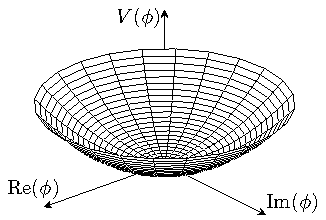
\includegraphics[width=\textwidth]{figures/higgs_potential_miu_0.pdf}
    \caption{$\mu^2 < 0$}
\end{subfigure}
\hfill
\begin{subfigure}[b]{0.48\textwidth}
    \centering
    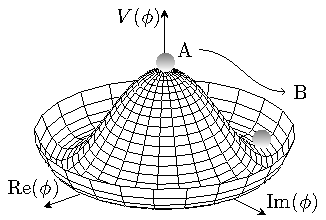
\includegraphics[width=\textwidth]{figures/higgs_potential.pdf}
    \caption{$\mu^2 > 0$}
\end{subfigure}
\caption{
The illustration of Higgs potential $V(\phi)$. 
Point B represents the non-zero vacuum expectation value (VEV) of the field.
Adapted from Ref.~\cite{TikZNetHiggsPotential}.
}
\label{fig:higgs_potential}

\end{figure}

The only transformation that leaves this vacuum invariant corresponds to the electromagnetic $\mathrm{U}(1)_{\mathrm{EM}}$. 
This spontaneously breaks the electroweak symmetry as $\mathrm{SU}(2)_L \times \mathrm{U}(1)_Y \;\rightarrow\; \mathrm{U}(1)_{\mathrm{EM}}$, 
and identifies the electric charge operator 
\[
Q = T_{3} + \frac{Y}{2},
\]
which generates the unbroken electromagnetic symmetry.

Expanding the Higgs field around the vacuum shows that three would-be Goldstone bosons emerge, corresponding to the broken generators. 
In a gauge theory, these Goldstone modes are absorbed by the gauge fields, providing the longitudinal components of the massive vector bosons. 
The covariant derivative acting on $\phi$,

\begin{equation}
    D_\mu \phi
    = \left( \partial_\mu 
    - i g T^i W_\mu^i
    - i g' \frac{Y}{2} B_\mu \right) \phi,
\end{equation}

generates mass terms for the weak gauge bosons once $\phi$ is replaced by its VEV. 
Diagonalising the resulting fields leads to the physical combinations

\begin{align}
    W_\mu^\pm &= \frac{1}{\sqrt{2}} (W_\mu^1 \mp i W_\mu^2), \\
    Z_\mu &= \cos\theta_W\, W_\mu^3 - \sin\theta_W\, B_\mu, \\
    A_\mu &= \sin\theta_W\, W_\mu^3 + \cos\theta_W\, B_\mu,
\end{align}

where $\theta_W$ is the weak mixing angle. 
The $W^\pm$ and $Z$ bosons acquire masses

\begin{equation}
    m_W = \frac{1}{2} g v, 
    \qquad
    m_Z = \frac{1}{2}\sqrt{g^2 + g'^2}\, v,
\end{equation}

while the photon remains massless, corresponding to the unbroken electromagnetic symmetry.
The fact that the Higgs field is a singlet under $\mathrm{SU}(3)_c$ leads directly to a massless gluon.

After absorbing three Goldstone modes, one physical scalar degree of freedom remains: the Higgs boson $h(x)$, with mass

\begin{equation}
    m_h = \sqrt{2\lambda}\, v.
\end{equation}

Thus, the BEH mechanism successfully explains the origin of electroweak gauge boson masses while preserving the gauge invariance and renormalisability of the theory.
Then the task is to generate fermion masses, which is accomplished through Yukawa interactions with the Higgs field:

\begin{equation}
\mathcal{L}_\text{Yukawa} = - y_d \, \bar{Q}_L \phi \, d_R
                - y_u \, \bar{Q}_L \tilde{\phi} \, u_R
                - y_e \, \bar{L}_L \phi \, e_R
                + \text{h.c.},
\end{equation}\label{eq:SM-Yukawa}

where $Q_L$ and $L_L$ are the left-handed quark and lepton doublets, $u_R$, $d_R$, and $e_R$ are the right-handed singlets, 
$\tilde{\phi} = i\sigma_2 \phi^*$, and $y_f$ are the Yukawa couplings. 
When the Higgs field acquires its vacuum expectation value $\langle \phi \rangle = (0, v/\sqrt{2})^T$, these terms generate fermion masses

\begin{equation}
m_f = \frac{y_f v}{\sqrt{2}}.
\end{equation}

In the quark sector, the Yukawa couplings are generally non-diagonal in flavor space, leading to mixing between different generations. 
After rotating the quark fields to mass eigenstates, the misalignment between the up-type and down-type Yukawa matrices gives rise to the Cabibbo-Kobayashi-Maskawa (CKM) matrix~\cite{Cabibbo1963,KobayashiMaskawa1973}, 
which appears in the charged weak interactions:

\begin{equation}
\mathcal{L}_\text{charged current} = \frac{g}{\sqrt{2}} \, \bar{u}_L \gamma^\mu V_{\mathrm{CKM}} \, d_L \, W_\mu^+ + \text{h.c.}.
\end{equation}

\subsection{Standard Model in a Nutshell}
\label{subsec:full-lagrangian}

In the preceding sections, the individual building blocks of the Standard Model have been introduced:
the gauge-field dynamics governed by Yang--Mills theory,
the kinetic terms for chiral fermions,
the Higgs sector responsible for electroweak symmetry breaking,
and the Yukawa interactions generating fermion masses.
These ingredients can be assembled into a single, compact Lagrangian density that fully specifies the Standard Model at the renormalisable level,
\begin{equation}
\mathcal{L}_{\mathrm{SM}}
= \mathcal{L}_{\mathrm{gauge}}~\eqref{eq:SM-gauge}
+ \mathcal{L}_{\mathrm{fermion}}~\eqref{eq:SM-fermion}
+ \mathcal{L}_{\mathrm{Higgs}}~\eqref{eq:SM-Higgs}
+ \mathcal{L}_{\mathrm{Yukawa}}~\eqref{eq:SM-Yukawa}.
\end{equation}
Together with the gauge symmetry $G_{\mathrm{SM}}$ and the pattern of electroweak symmetry breaking,
this Lagrangian defines the complete particle content and interaction structure of the Standard Model,
which is schematically summarised in Fig.~\ref{fig:SM-table}.

The SM particle content is carefully arranged to ensure the cancellation of all gauge anomalies. This nontrivial condition relates the quantum numbers of quarks and leptons and partially explains the observed charge quantization.
This anomaly cancellation together with gauge symmetry and renormalisability impose strong theoretical constraints on the structure of the Standard Model, leaving remarkably little freedom in its formulation.
Within this framework, the particle content, interaction vertices, and symmetry-breaking pattern are largely fixed.
Over several decades, an extensive programme of experimental tests has confirmed the predictions of the Standard Model to a high degree of accuracy. Key milestones include the discovery of weak neutral currents at Gargamelle~\cite{Hasert1973}, the observation of $W$ and $Z$ bosons at the SPS~\cite{UA1_1983,UA2_1983}, precision electroweak measurements at LEP and SLC~\cite{LEP2006}, the observation of the top quark at Tevatron~\cite{CDF1995, D01995}, the discovery of the Higgs boson at the LHC and subsequent precision studies of its couplings~\cite{ATLAS_CMS_Higgs2022}.
% Despite this success, the Standard Model is widely regarded as an effective description valid up to a finite energy scale, motivating ongoing experimental and theoretical efforts to search for deviations and to explore physics beyond the Standard Model.

\begin{figure}[!t]
    \centering
        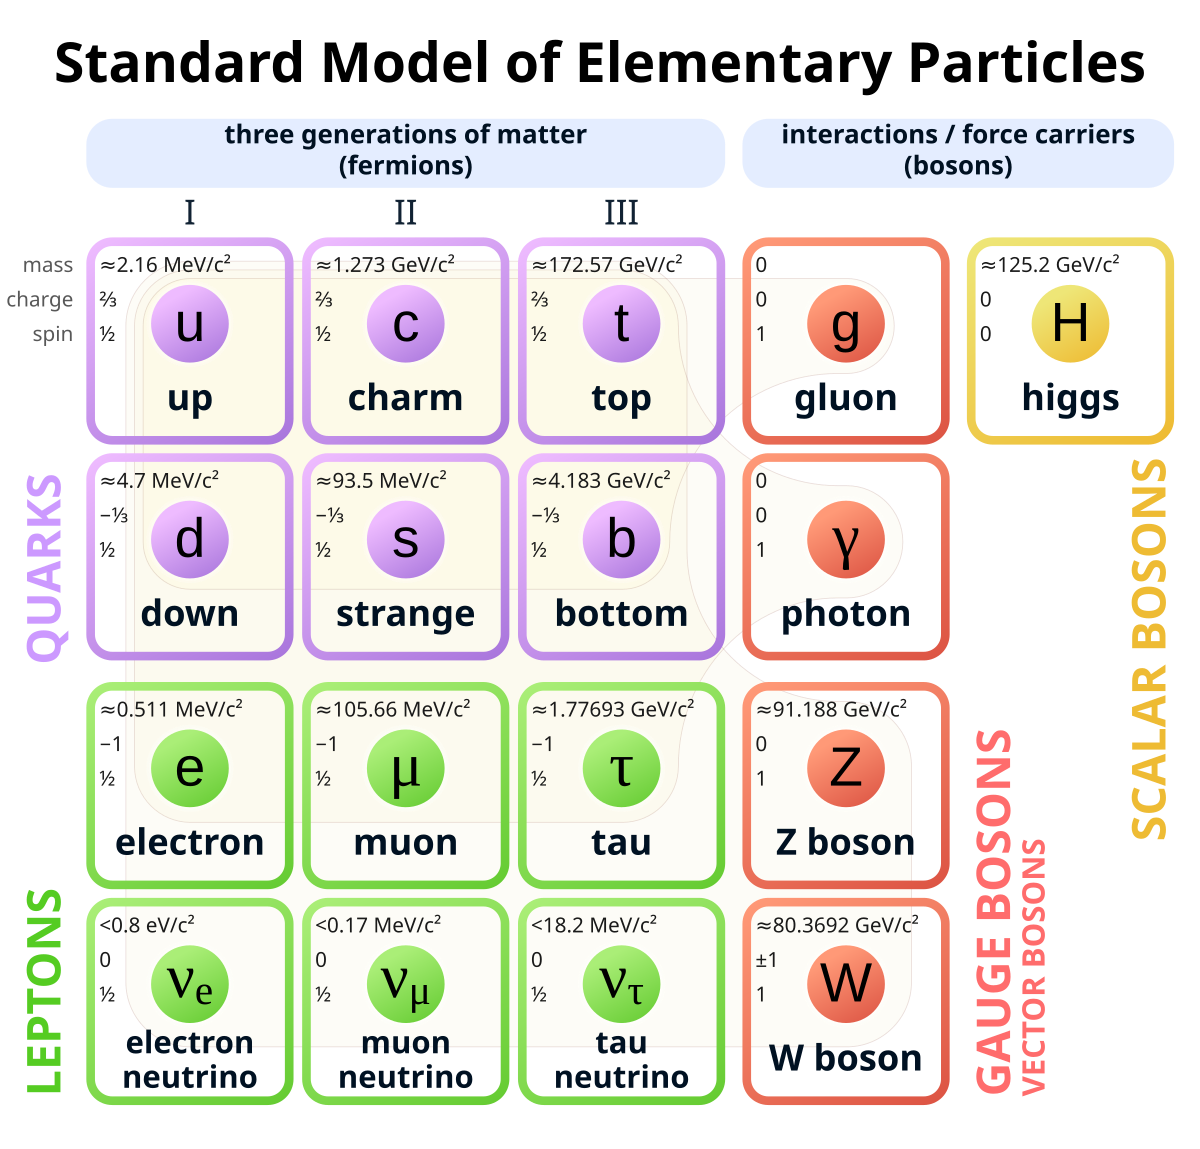
\includegraphics[width=0.9\textwidth]{figures/Standard_Model.png}
    \caption{A schematic overview of the particle content of the Standard Model.
    Fermions come in three generations, gauge bosons mediate the interactions,
    and the Higgs field provides masses through electroweak symmetry breaking.}
    \label{fig:SM-table}
\end{figure}

\section{Beyond the Standard Model}\label{sec:BSM}

Despite its tremendous success in matching experimental results over decades, the Standard Model is known to be incomplete.
Thus, various extensions have been proposed to address its limitations and open questions.

\subsection{Limitations of the Standard Model}\label{subsec:limitations}

One of the most evident omissions of the Standard Model is that it
does not incorporate gravity. While the SM is formulated as a quantum
field theory based on local gauge symmetries, gravity is described by
general relativity~\cite{Einstein1916GR}, a classical theory of curved
spacetime. A straightforward quantisation of gravity leads to a
non-renormalisable theory, indicating that a more fundamental
framework is required to unify gravity with the other interactions.
Astrophysical and cosmological observations also reveal that ordinary
baryonic matter constitutes only a small fraction of the total energy
density of the Universe, while dark matter and dark energy together
account for about 95\% of it~\cite{Begeman1991RotationCurves,PlanckXVI2014CosmologicalParameters}.
However, the SM contains no viable dark matter candidate and provides
no explanation for the accelerated expansion of the Universe.

Several experimental observations further indicate physics beyond the
Standard Model. Neutrino oscillation experiments have demonstrated
that neutrinos possess small but non-zero masses~\cite{Fukuda1998NeutrinoOscillation},
which cannot be accommodated within the minimal SM. In addition,
the observed baryon asymmetry of the Universe requires mechanisms
satisfying the Sakharov conditions~\cite{Sakharov:1967dj}: baryon
number violation, C and CP violation, and departure from thermal
equilibrium. Although the SM contains CP violation through the CKM
matrix, it is insufficient to explain the observed asymmetry.

The Standard Model also faces theoretical challenges, notably the
hierarchy problem~\cite{Veltman1981,PeskinHierarchy}. While the SM
successfully describes particle interactions at currently accessible
energies, it does not explain why the electroweak scale,
$v \simeq 246~\mathrm{GeV}$, is vastly smaller than the Planck scale,
$M_{\mathrm{Pl}} \sim 10^{19}~\mathrm{GeV}$. The Higgs boson receives
large radiative corrections to its mass parameter. At one loop the
quadratically divergent correction can be written schematically as

\begin{equation}
\delta m_H^2 \sim
\frac{\Lambda^2}{16\pi^2}
\left(
6\lambda + \frac{9}{4}g^2 + \frac{3}{4}g'^2 - 6y_t^2
\right),
\end{equation}

where $\Lambda$ denotes the cutoff scale of the theory. The
top-quark contribution dominates due to its large Yukawa coupling.
If the SM remains valid up to very high scales such as the Planck
scale, maintaining the observed Higgs boson mass
$m_H \simeq 125~\mathrm{GeV}$ requires a delicate cancellation between
the bare mass parameter and the quantum corrections, leading to a
fine-tuning problem. More broadly, this issue may be viewed as
encompassing three related aspects: the large hierarchy between the
electroweak and Planck scales, the special status of scalar fields
whose masses are not protected by symmetries, and the so-called
``little hierarchy problem'' associated with the absence of new
physics at the TeV scale~\cite{PeskinHierarchy}. Taken together,
these considerations have long motivated the expectation that new
physics may appear near the TeV scale.

\subsection{Two-Higgs-Doublet Model}\label{subsec:2HDM}

The Two-Higgs-Doublet Model (2HDM~\cite{Branco:2011iw}) represents one of the simplest and
best-motivated extensions of the SM scalar sector.
One of the strongest theoretical motivations for the Two-Higgs-Doublet
Model arises from supersymmetry, where two Higgs doublets are required
both to generate masses for up- and down-type fermions and to ensure
anomaly cancellation in the Minimal Supersymmetric Standard Model
Furthermore, the extended scalar sector can provide additional
sources of CP violation that may enable electroweak baryogenesis~\cite{Branco:2011iw}.
Additional motivation arises in Peccei--Quinn axion models addressing
the strong CP problem~\cite{Peccei:1977hh,Peccei:1977ur}.
Together, these considerations establish the 2HDM as a minimal yet
well-motivated framework for exploring physics beyond the Standard Model.

The 2HDM extends the Standard Model by introducing two complex
$\mathrm{SU}(2)_L$ scalar doublets with hypercharge $Y=+1/2$,
\[
\Phi_i =
\begin{pmatrix}
\phi_i^+ \\
\frac{1}{\sqrt{2}}(v_i + \rho_i + i \eta_i)
\end{pmatrix},
\qquad i = 1,2,
\]
whose vacuum expectation values satisfy
\[
v^2 \equiv v_1^2 + v_2^2 = (246~\mathrm{GeV})^2 .
\]
It is customary to define the ratio of the two vacuum expectation values as
$\tan\beta \equiv v_2 / v_1$.

The most general renormalisable scalar potential involving the two
doublets contains several quadratic and quartic couplings as well as
possible soft symmetry-breaking terms.
In phenomenological studies it is common to trade these parameters for
the physical Higgs masses, the mixing angles $\alpha$ and $\beta$,
and the soft-breaking scale.

After electroweak symmetry breaking, the eight scalar degrees of
freedom contained in the two doublets reorganise into five physical
Higgs bosons and three Goldstone bosons absorbed by the electroweak
gauge bosons.
The charged scalar fields $\phi_1^\pm$ and $\phi_2^\pm$ mix to form a
pair of physical charged Higgs bosons $H^\pm$ and the charged
Goldstone bosons $G^\pm$, while the neutral CP-odd fields $\eta_1$
and $\eta_2$ mix into the pseudoscalar Higgs boson $A$ and the
neutral Goldstone boson $G^0$.

In the CP-even sector, the neutral fields $\rho_1$ and $\rho_2$
mix to form two physical scalar mass eigenstates, conventionally
denoted by $h$ and $H$,
\[
\begin{pmatrix}
H \\
h
\end{pmatrix}
=
\begin{pmatrix}
\cos\alpha & \sin\alpha \\
-\sin\alpha & \cos\alpha
\end{pmatrix}
\begin{pmatrix}
\rho_1 \\
\rho_2
\end{pmatrix},
\]
where $\alpha$ is the CP-even Higgs mixing angle.
The lighter CP-even state $h$ is typically identified with the
observed Higgs boson with a mass of approximately $125~\mathrm{GeV}$, while $H$, $A$, and
$H^\pm$ correspond to additional scalar states predicted by the
2HDM.

The interactions between the Higgs doublets and fermions are
described by the Yukawa sector.
In the most general renormalisable form, both Higgs doublets can
couple to a given fermion species, leading to
\[
\begin{aligned}
\mathcal{L}_\text{Yukawa} =\;&
- \bar{Q}_L \left( Y_1^u \tilde{\Phi}_1 + Y_2^u \tilde{\Phi}_2 \right) u_R
- \bar{Q}_L \left( Y_1^d \Phi_1 + Y_2^d \Phi_2 \right) d_R \\
&- \bar{L}_L \left( Y_1^\ell \Phi_1 + Y_2^\ell \Phi_2 \right) \ell_R
+ \text{h.c.},
\end{aligned}
\]
where $\tilde{\Phi}_i = i \sigma_2 \Phi_i^\ast$.
In this general case, tree-level flavour-changing neutral currents
(FCNCs) arise after electroweak symmetry breaking.
To avoid this, a discrete $\mathbb{Z}_2$ symmetry is commonly
imposed, ensuring that each fermion type couples to only one
Higgs doublet, a condition known as natural flavour conservation.

Imposing such a symmetry leads to several phenomenologically
distinct realisations of the 2HDM, classified according to the
Higgs doublet responsible for generating the masses of different
fermion species.
The commonly considered Yukawa types are summarised in
Table~\ref{tab:2hdm_yukawa_types}.

\begin{table}[htbp]
\centering
\caption{Yukawa coupling assignments in 2HDMs with natural flavour
conservation obtained by imposing a discrete $\mathbb{Z}_2$ symmetry.}
\begin{tabular}{c|ccc}
\hline
Type & Up-type quarks & Down-type quarks & Charged leptons \\
\hline
Type-I  & $\Phi_2$ & $\Phi_2$ & $\Phi_2$ \\
Type-II & $\Phi_2$ & $\Phi_1$ & $\Phi_1$ \\
Type-X (Lepton-specific) & $\Phi_2$ & $\Phi_2$ & $\Phi_1$ \\
Type-Y (Flipped) & $\Phi_2$ & $\Phi_1$ & $\Phi_2$ \\
\hline
\end{tabular}
\label{tab:2hdm_yukawa_types}
\end{table}

In this thesis we focus on the Type-II 2HDM, in which up-type quarks
couple exclusively to $\Phi_2$, while down-type quarks and charged
leptons couple to $\Phi_1$.
The corresponding Yukawa Lagrangian is given by
\[
\mathcal{L}_\text{Yukawa}^{\text{Type-II}} =
- \bar{Q}_L Y_u \tilde{\Phi}_2 u_R
- \bar{Q}_L Y_d \Phi_1 d_R
- \bar{L}_L Y_\ell \Phi_1 \ell_R
+ \text{h.c.}.
\]

After electroweak symmetry breaking, the fermion masses are generated as
\[
m_u = \frac{Y_u v_2}{\sqrt{2}}, \qquad
m_d = \frac{Y_d v_1}{\sqrt{2}}, \qquad
m_\ell = \frac{Y_\ell v_1}{\sqrt{2}},
\]
making the dependence on $\tan\beta$ explicit.

Current Higgs measurements indicate that the observed
$125~\mathrm{GeV}$ Higgs boson closely resembles the Standard Model
Higgs, which corresponds in the 2HDM to the alignment limit
$\sin(\beta-\alpha) \to 1$.
In this regime the couplings of the light Higgs boson $h$ approach
their SM values.
For the heavier neutral Higgs bosons $H$ and $A$, the Yukawa
couplings depend strongly on $\tan\beta$.
In the Type-II scenario the couplings to up-type quarks scale
approximately as $1/\tan\beta$, while those to down-type fermions
scale as $\tan\beta$.
Consequently, at small values of $\tan\beta$ the interactions with
top quarks can become significantly enhanced.
Processes involving top quarks therefore provide a particularly
sensitive probe of the extended Higgs sector, motivating searches
in multi-top final states.

\subsection{Top-Philic Simplified Models}\label{subsec:S1/S8}

The top quark occupies a unique position within the SM, 
as will be discussed in more detail in Section~\ref{sec:four-tops}. 
With a mass close to the electroweak symmetry-breaking scale, the top quark 
is expected to play a special role in many theories extending the SM. 
Consequently, a wide range of new-physics scenarios predict additional 
degrees of freedom that couple preferentially to the top quark. 
From an experimental perspective, processes involving multiple top quarks 
probe the highest energy scales accessible at the Large Hadron Collider (LHC) 
and therefore provide a particularly sensitive window to such interactions.

While many ultraviolet (UV) complete models predict new interactions in the~\cite{BattagliaServant2010FourTop,LillieShuTait2008TopCompositeness,Gerbush2008ColorOctet,SalamStrathdee1975SUSYFermionNumber}
top sector, their detailed particle content and coupling structures are often 
too model-dependent to be directly tested at colliders. 
An alternative description is provided by the Standard Model Effective Field 
Theory (SMEFT), where the effects of heavy new physics are parametrised through 
higher-dimensional operators~\cite{Agram2013TopAnomalous,DHondt2018PinpointOperators,Banelli2021FourTopOperators}. 
However, the SMEFT expansion assumes that the characteristic new-physics scale 
is significantly larger than the typical energy scale probed by the process. 
In multi-top final states, the partonic centre-of-mass energy can reach the 
TeV scale, and the validity of the EFT expansion may therefore become questionable. 
In this regime, the EFT approach may fail to capture resonant or kinematic 
effects associated with the direct production of new particles.

To bridge the gap between UV-complete models and the EFT description, 
top-philic simplified models provide a convenient intermediate framework~\cite{Darme:2021gtt}. 
These models aim to capture the leading phenomenological consequences of a 
broad class of theories by introducing only the minimal set of new degrees of 
freedom relevant for collider observables. 
In practice, the SM particle content is extended by a single heavy mediator 
that couples predominantly to top quarks, while the number of free parameters 
is kept small to maintain a transparent interpretation of experimental results.

The construction of these models is guided by general symmetry considerations. 
Requiring invariance under the residual gauge symmetry 
$SU(3)_\mathrm{C} \times U(1)_\mathrm{em}$ and renormalisable interactions 
with top-quark bilinears restricts the mediator to be either a scalar or a 
vector particle transforming as a colour singlet or colour octet. 
This leads to four generic classes of top-philic mediators: scalar singlets 
($S_1$), scalar octets ($S_8$), vector singlets ($V_1$), and vector octets ($V_8$).

At the Lagrangian level, the interaction between a scalar mediator and the 
top quark can be written as
\begin{equation}
\mathcal{L}_{\text{scalar}} \supset
-\frac{1}{2} m_S^2 S S
- y_S\, S\, \bar{t}\left(\cos\phi + i\gamma_5\sin\phi\right)t ,
\end{equation}
for a colour-singlet mediator. 
For a colour-octet scalar $S^a$, the interaction involves the generators 
$T^a$ of $SU(3)_\mathrm{C}$,
\begin{equation}
\mathcal{L}_{\text{scalar}} \supset
-\frac{1}{2} m_S^2 S^a S^a
- y_S\, S^a\, \bar{t}T^a\left(\cos\phi + i\gamma_5\sin\phi\right)t .
\end{equation}
The mixing angle $\phi$ parametrises the relative scalar and pseudoscalar 
components of the interaction.

For a vector mediator, the interaction with the top quark can be written as
\begin{equation}
\mathcal{L}_{\text{vector}} \supset
-\frac{1}{4} V^a_{\mu\nu} V^{a\,\mu\nu}
+ \frac{1}{2} m_V^2 V^a_\mu V^{a\,\mu}
+ g_t\, V^a_\mu\, \bar{t}\gamma^\mu
(c_L P_L + c_R P_R) T^a t ,
\end{equation}
where $P_{L,R}$ denote the chirality projection operators and the parameters 
$c_L$ and $c_R$ determine the chiral structure of the interaction. 
For colour-singlet mediators, the generator $T^a$ is replaced by the identity.

The four classes of mediators considered in this work are summarised in 
Table~\ref{tab:mediators}. 
Together, these simplified models provide a minimal and systematic 
parameterisation of possible new physics effects in the top sector while 
keeping the number of free parameters small.

\begin{table}[htbp]
\centering
\begin{tabular}{cccc}
\hline
Mediator & Spin & Colour & Coupling to top quark \\
\hline
$S_1$ & 0 & 1 & $y_S\,S\,\bar{t}(\cos\phi+i\gamma_5\sin\phi)t$ \\
$S_8$ & 0 & 8 & $y_S\,S^a\,\bar{t}T^a(\cos\phi+i\gamma_5\sin\phi)t$ \\
$V_1$ & 1 & 1 & $g_t\,V_\mu\,\bar{t}\gamma^\mu(c_LP_L+c_RP_R)t$ \\
$V_8$ & 1 & 8 & $g_t\,V^a_\mu\,\bar{t}\gamma^\mu(c_LP_L+c_RP_R)T^a t$ \\
\hline
\end{tabular}
\caption{Classification of top-philic simplified mediators considered in this work.}
\label{tab:mediators}
\end{table}

A key phenomenological difference between colour-singlet and colour-octet 
mediators arises from their production mechanisms at hadron colliders. 
While colour-singlet states are produced primarily through their couplings 
to top quarks, colour-octet mediators can additionally be pair-produced via 
QCD interactions, leading to potentially larger production cross-sections.

In the limit where the mediator mass is much larger than the characteristic 
energy scale of the process, these simplified models can be matched onto 
higher-dimensional four-fermion operators in the EFT description. 
However, for mediator masses in the TeV range, which are directly accessible 
at the LHC, it is essential to retain the explicit mediator degrees of freedom 
in order to correctly describe resonant production and the associated 
kinematic features.

\section{Top Quarks and Four-Tops Production}
\label{sec:four-tops}

In the preceding sections, the theoretical structure of the Standard Model and several well-motivated extensions
have been introduced, with particular emphasis on the gauge sector, the mechanism of electroweak symmetry breaking,
and models featuring extended scalar sectors or enhanced couplings to the top quark.
To conclude this theoretical overview, we now focus on the top quark and on processes involving multiple top quarks,
which provide a natural meeting point between the Standard Model dynamics and many of the beyond-the-Standard-Model
scenarios discussed above.

Among the multi-top final states accessible at the Large Hadron Collider,
the production of four top quarks,
$pp \to t\bar{t}t\bar{t}$,
occupies a special role due to its high kinematic threshold and its sensitivity to strong, electroweak,
and Yukawa interactions.
Before discussing the mechanisms contributing to four-tops production,
the key properties of the top quark are briefly summarised.

\subsection{Top-quark properties}
\label{subsec:top_properties}

The top quark was discovered in 1995 by the CDF~\cite{CDF1995} and D0~\cite{D01995} collaborations at the Fermilab Tevatron,
completing the third generation of quarks predicted by the Standard Model.
Its discovery confirmed the quark-sector structure of the Standard Model
and revealed a fermion with a mass unexpectedly close to the electroweak scale.
This striking feature immediately distinguished the top quark from all other known fermions
and motivated extensive studies of its role in electroweak symmetry breaking
and in physics beyond the Standard Model.

The top quark is the third-generation up-type fermion of the Standard Model,
carrying spin $1/2$ and electric charge $+2/3$.
It transforms as a colour triplet under $\mathrm{SU}(3)_C$
and forms an $\mathrm{SU}(2)_L$ weak isospin doublet together with the bottom quark.
Apart from its mass, all gauge quantum numbers of the top quark
are identical to those of the lighter up-type quarks.

The defining property of the top quark is its exceptionally large mass,
$m_t \simeq 173~\mathrm{GeV}$,
which lies close to the electroweak scale.
Within the Standard Model, this mass originates from a Yukawa interaction with the Higgs field,
\begin{equation}
m_t = \frac{y_t v}{\sqrt{2}},
\end{equation}
where $v \simeq 246~\mathrm{GeV}$ is the Higgs vacuum expectation value.
The corresponding Yukawa coupling $y_t$ is of order unity,
making the top quark unique among the fermions of the Standard Model.
As a consequence, the top quark plays a central role in radiative corrections to the Higgs potential
and in the renormalisation-group evolution of Standard Model parameters.

Another distinctive feature of the top quark is its extremely short lifetime,
which is shorter than the typical timescale for hadronisation.
The top quark therefore decays before forming bound states,
predominantly via the weak transition $t \to W b$.
This property allows information about the top-quark spin and interaction structure
to be directly transferred to its decay products,
enabling detailed experimental studies of top-quark couplings and polarisation effects.

Owing to its large mass and strong coupling to the Higgs sector,
the top quark is particularly sensitive to modifications of the electroweak and scalar sectors.
Processes involving multiple top quarks probe the top sector at high energy scales
and can receive sizeable contributions from extensions of the Standard Model
that introduce new degrees of freedom coupled to the top quark.
In this context, the production of four top quarks provides a natural framework
for studying the interplay between strong, electroweak, and Yukawa interactions,
as discussed in the following sections.

\subsection{Four-Tops Production in the Standard Model}

The production of four top quarks, $pp \to t\bar{t}t\bar{t}$, constitutes one of the rarest processes predicted by the Standard Model at the Large Hadron Collider.
Its small production rate is a consequence of both the large energy threshold required to produce four heavy quarks and the high perturbative order involved.
Despite its rarity, four-tops production occupies a unique position in collider phenomenology, 
as it probes the top quark sector at the highest accessible energy scales and is simultaneously sensitive to strong, electroweak, and Yukawa interactions~\cite{Blekman2022FourTopLHC}.

At leading order, four-tops production proceeds predominantly through QCD-mediated processes. 
Representative Feynman diagrams include gluon exchange, top-quark exchange, and box-type topologies. 
In addition to the pure QCD contribution, subleading electroweak diagrams involving $\gamma$, $Z$ or Higgs boson exchange also contribute, as well as interference terms between QCD and electroweak amplitudes.
In Figure~\ref{fig:four-tops-schematic}, two representative diagrams are illustrated.

% ========== SM four-tops (schematic) ==========
\begin{figure}[htbp]
\centering
\begin{subfigure}[b]{0.45\textwidth}
\centering
\begin{tikzpicture}
\begin{feynman}

    % incoming gluons
    \vertex (g1) at (-2,1) {\(g\)};
    \vertex (g2) at (-2,-1) {\(g\)};

    % production vertices
    \vertex (v1) at (0,1);
    \vertex (v2) at (0,-1);

    % t-channel exchange
    \vertex (vx1) at (0.5,0.6);
    \vertex (vx2) at (0.5,-0.6);

    % outgoing tops left pair
    \vertex (t1) at (2.5,1.8) {\(t\)};
    \vertex (tb1) at (2.5,0.6) {\(\bar t\)};

    % outgoing tops right pair
    \vertex (t2) at (2.5,-0.6) {\(t\)};
    \vertex (tb2) at (2.5,-1.8) {\(\bar t\)};

    % diagram
    \diagram*{

      % initial gluon fusion
      (g1) -- [gluon] (v1),
      (g2) -- [gluon] (v2),

      % left ttbar production
      (v1) -- [fermion] (t1),
      (v1) -- [anti fermion] (vx1),

      % right ttbar production
      (v2) -- [anti fermion] (tb2),
      (v2) -- [fermion] (vx2),

      % t-channel gluon exchange
      (vx1) -- [gluon] (vx2),

      % final outgoing particles
      (vx1) -- [fermion] (tb1),
      (vx2) -- [anti fermion] (t2),
    };
\end{feynman}
\end{tikzpicture}
\end{subfigure}
\hfill

\begin{subfigure}[b]{0.45\textwidth}
\centering
\begin{tikzpicture}
\begin{feynman}

    % gluons
    \vertex (g1) at (-2,1.5) {\(g\)};
    \vertex (g2) at (-2,-1.5) {\(g\)};

    % initial ttbar
    \vertex (v1) at (-0.5,1);
    \vertex (v2) at (-0.5,-1);

    % heavy Higgs line
    \vertex (hmid) at (0.5,0);
    \vertex (hlabel) at (1.5,0);

    % final ttbar from H/A decay
    \vertex (t1) at (3,0.8) {\(t\)};
    \vertex (tb1) at (3,-0.8) {\(\bar t\)};

    % spectator ttbar
    \vertex (ts) at (2.4,1.8) {\(t\)};
    \vertex (tbs) at (2.4,-1.8) {\(\bar t\)};

    \diagram*{
      % initial gluons
      (g1) -- [gluon] (v1),
      (g2) -- [gluon] (v2),

      % spectator ttbar
      (v1) -- [fermion] (ts),
      (v2) -- [anti fermion] (tbs),

      % two internal tops → H
      (v1) -- [anti fermion] (hmid),
      (v2) -- [fermion] (hmid),

      % H production
      (hmid) -- [scalar, dashed, edge label=\(H\)] (hlabel),

      % H decay → ttbar
      (hlabel) -- [fermion] (t1),
      (hlabel) -- [anti fermion] (tb1),
    };

\end{feynman}
\end{tikzpicture}
\end{subfigure}
\caption{Illustration of the Standard Model four-tops production The mediator connecting two top quarks can be a gluon, a neutral electroweak gauge boson ($\gamma$ or $Z$), or a Higgs boson.
.}
\label{fig:four-tops-schematic}
\end{figure}

Although the Higgs-mediated contribution represents only a small fraction of the total cross section, it introduces a direct dependence on the top Yukawa coupling.
As a result, four-tops production provides a complementary probe of the top-Higgs interaction beyond processes such as inclusive $t\bar{t}$ or associated $t\bar{t}H$ production.

Next-to-leading-order calculations predict a Standard Model cross section of approximately $\sigma(pp \to t\bar{t}t\bar{t}) = 13.4^{+1.0}_{-1.8}~\mathrm{fb}$ at a centre-of-mass energy of $\sqrt{s}=13~\mathrm{TeV}$~\cite{vanBeekveld:2022hty}.
This value is more than four orders of magnitude smaller than the inclusive $t\bar{t}$ production cross section, highlighting the experimental challenges associated with observing this process.

\subsection{BSM Contributions to Four-Tops Production}

The four-tops final state is particularly sensitive to new physics scenarios that feature enhanced couplings to the top quark. 
In the following, two representative models introduced earlier in this thesis are discussed: the two-Higgs-doublet model (2HDM) with heavy neutral scalars, and models containing a colour-octet scalar ($S_{8}$).
Their characteristic contributions to four-tops production are illustrated in Fig.~\ref{fig:bsm_4top_feynman}.

\paragraph{Four-Tops production in 2HDM.}
In the 2HDM, the presence of additional heavy neutral Higgs bosons, a CP-even scalar \(H\) and a CP-odd pseudoscalar \(A\), provides new resonant contributions to four-tops production. 
As illustrated in Fig.~\ref{fig:HAtotttt}, the dominant mechanism proceeds via gluon-initiated top-quark pair production,
where an internal \(t\bar{t}\) pair radiates a heavy scalar \(H/A\), which subsequently decays into a second \(t\bar{t}\) pair.

This contribution is strongly enhanced by the large top Yukawa coupling. In particular, in the alignment limit where the light Higgs boson behaves SM-like, 
the couplings of \(H/A\) to top quarks can be significantly increased, especially at low values of \(\tan\beta\).
When the heavy scalar mass satisfies \(m_{H/A} > 2m_t\), the decay \(H/A \to t\bar{t}\) becomes dominant, leading to a resonant enhancement of the four-tops production cross section.

\paragraph{Four-top production via $S_{8}$.}
\label{sec:sgluon_tttt}

The $S_{8}$ transforms in the adjoint representation
of \(\mathrm{SU}(3)_\mathrm{c}\) and therefore interacts strongly with gluons.
As illustrated in Fig.~\ref{fig:sgluontotttt}, pairs of $S_{8}$s can be produced efficiently at the LHC through
gluon--gluon fusion and quark--antiquark annihilation,
\(pp \rightarrow S_8 S_8\).
Owing to the strong production mechanism, the production cross section
is largely determined by QCD interactions and depends mainly on the
$S_{8}$ mass.
If the $S_{8}$ couples preferentially to top quarks,
its dominant decay mode is \(S_8 \rightarrow t\bar{t}\).
The pair production process therefore leads to a four-top final state
\(pp \rightarrow S_8 S_8 \rightarrow t\bar{t}t\bar{t}\).

In simplified models, the coupling of the $S_{8}$ to top quarks is
parameterised by a Yukawa-like coupling \(y_{S_8}\).
For moderate values of this coupling, the dominant contribution to the
four-top final state arises from $S_{8}$ pair production followed by the
decay \(S_8\rightarrow t\bar{t}\).
Additional processes such as associated production
(\(pp \rightarrow t\bar{t}S_8\)) and interference with the Standard Model
background are typically subleading for \(y_{S_8}\lesssim 0.1\).

In contrast to the 2HDM case, where four-top production arises from the
decay of a single heavy resonance, the $S_{8}$ scenario involves the
on-shell production of two heavy coloured particles.
The resulting topology therefore features two resonant
\(t\bar{t}\) systems and typically exhibits large hadronic activity and
high jet multiplicity in the final state.

\begin{figure}[htbp]
\centering
% ------------------ 2HDM HEAVY HIGGS ------------------
\begin{subfigure}[t]{0.45\textwidth}
\centering
\begin{tikzpicture}
\begin{feynman}

    % gluons
    \vertex (g1) at (-2,1.5) {\(g\)};
    \vertex (g2) at (-2,-1.5) {\(g\)};

    % initial ttbar
    \vertex (v1) at (-0.5,1);
    \vertex (v2) at (-0.5,-1);

    % heavy Higgs line
    \vertex (hmid) at (0.5,0);
    \vertex (hlabel) at (1.5,0);

    % final ttbar from H/A decay
    \vertex (t1) at (3,0.8) {\(t\)};
    \vertex (tb1) at (3,-0.8) {\(\bar t\)};

    % spectator ttbar
    \vertex (ts) at (2.4,1.8) {\(t\)};
    \vertex (tbs) at (2.4,-1.8) {\(\bar t\)};

    \diagram*{
      % initial gluons
      (g1) -- [gluon] (v1),
      (g2) -- [gluon] (v2),

      % spectator ttbar
      (v1) -- [fermion] (ts),
      (v2) -- [anti fermion] (tbs),

      % two internal tops → H/A
      (v1) -- [anti fermion] (hmid),
      (v2) -- [fermion] (hmid),

      % H/A production
      (hmid) -- [scalar, dashed, edge label=\(H/A\)] (hlabel),

      % H/A decay → ttbar
      (hlabel) -- [fermion] (t1),
      (hlabel) -- [anti fermion] (tb1),
    };

\end{feynman}
\end{tikzpicture}
\caption{2HDM: \(H/A\) produced from internal \(t\bar t\), decaying to \(t\bar t\).}
\label{fig:HAtotttt}
\end{subfigure}
\hfill
% ------------------ SGluon ------------------
\begin{subfigure}[t]{0.45\textwidth}
\centering
\begin{tikzpicture}
\begin{feynman}

    % incoming gluons
    \vertex (g1) at (-2,1.2) {\(g\)};
    \vertex (g2) at (-2,-1.2) {\(g\)};

    % sgluon pair
    \vertex (s1) at (-0.5,0);
    \vertex (s2) at (-0.5,0);
    \vertex (slabel1) at (1,0.6);
    \vertex (slabel2) at (1,-0.6);

    % ttbar from sgluon decays
    \vertex (t1) at (2.4,1.5) {\(t\)};
    \vertex (tb1) at (2.4,0.3) {\(\bar t\)};
    \vertex (t2) at (2.4,-0.3) {\(t\)};
    \vertex (tb2) at (2.4,-1.5) {\(\bar t\)};

    \diagram*{
      % gluon → sgluon pair
      (g1) -- [gluon] (s1),
      (g2) -- [gluon] (s2),

      % sgluon production
      (s1) -- [scalar, dashed, edge label=\(S_8\)] (slabel1),
      (s2) -- [scalar, dashed, edge label'=\(S_8\)] (slabel2),

      % sgluon decays to ttbar
      (slabel1) -- [fermion] (t1),
      (slabel1) -- [anti fermion] (tb1),
      (slabel2) -- [fermion] (t2),
      (slabel2) -- [anti fermion] (tb2),
    };

\end{feynman}
\end{tikzpicture}
\caption{$S_{8}$ pair production, each \(S_8 \to t\bar t\).}
\label{fig:sgluontotttt}
\end{subfigure}

\caption{BSM contributions to four-tops production: (left) 2HDM heavy scalar \(H/A\); (right) $S_{8}$ pair decay.}
\label{fig:bsm_4top_feynman}
\end{figure}